\section{Background}
The model of the surface vessel is based in the hydrodynamic modeling presented in \cite{TFossen}, where the principal effects that need to be taken into account are described.

In this section, the different contributions are summarized and related to the vessel at hand.

\subsection{Reference Frames}
To describe the orientation and position of the surface vessel two coordinate frames are used, the body frame and an inertial frame. For operations in a local area, with longitude and latitude approximately constants (flat navigation) a NED system (North-East-Down) can be assumed as an inertial frame where Newton's physics will apply \cite[p. 17]{TFossen}.

To distinguish between the two frames, the body frame is denoted by a subindex "$_\mathrm{b}$", and the inertial frame with subindex "$_\mathrm{n}$". In \autoref{fig:refFrame}, a diagram of the surface vessel with the notation used can be seen.

\begin{figure}[H]
    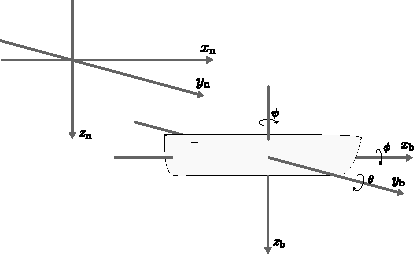
\includegraphics[width=0.6\textwidth]{figures/boat3D}
    \caption{$x_\mathrm{b}$, $y_\mathrm{b}$ and $z_\mathrm{b}$ refer to the position with respect to the body coordinate frame, while $x_\mathrm{n}$, $y_\mathrm{n}$ and $z_\mathrm{n}$ describe it with respect to the inertial frame. $\phi$, $\theta$ and $\psi$ refer to the rotation around $x_\mathrm{b}$, $y_\mathrm{b}$ and $z_\mathrm{b}$, respectively.}
    \label{fig:refFrame}
\end{figure}


The transformation from the body frame to the inertial can be done through a rotation matrix, \eqref{eq:RotMatrix}, which describes a total rotation in terms of three consecutive rotations.

In this case the rotation matrix is composed with a 1-2-3 convention, that is, first a rotation around $x_{\mathrm{b}}$, then around $y_{\mathrm{b}}$ and finally around $z_{\mathrm{b}}$ \cite[p. 22]{TFossen}.

\begin{minipage}{0.32\linewidth}
    \begin{flalign}
    \vec{R}_\mathrm{X} &=
    \begin{bmatrix}
    1 & 0      & 0       \\ 
    0 & c\phi  & -s\phi  \\ 
    0 & s\phi  & c\phi   \nonumber  
    \end{bmatrix} 	\label{eq:RotMatrix1}
    \end{flalign}
\end{minipage}\hfill
\begin{minipage}{0.32\linewidth}
    \begin{flalign}
    \vec{R}_\mathrm{Y} &=
    \begin{bmatrix}
    c\theta  & 0  & s\theta  \\ 
    0          & 1  & 0      \\ 
    -s\theta & 0  & c\theta  \nonumber 
    \end{bmatrix} 	\label{eq:RotMatrix2}
    \end{flalign}
\end{minipage}\hfill
\begin{minipage}{0.32\linewidth}
    \begin{flalign}
    \vec{R}_\mathrm{Z} &=
    \begin{bmatrix}
    c\psi & -s\psi  & 0  \\ 
    s\psi & c\psi   & 0  \\ 
    0       & 0         & 1  \nonumber 
    \end{bmatrix} 	\label{eq:RotMatrix3}
    \end{flalign}
\end{minipage}\hfill
\small
\begin{flalign}
\vec{R}^\mathrm{n}_\mathrm{b} = \vec{R}_Z \vec{R}_Y \vec{R}_X =
\begin{bmatrix}
c\theta c\psi  & s\phi s\theta c\psi -c\phi s\psi  & c\phi s\theta c\psi + s\phi s\psi  \\ 
c\theta s\psi  & s\phi s\theta s\psi + c\phi c\psi & c\phi s\theta s\psi - s\phi c\psi  \\ 
-s\theta         & s\phi c\theta                           & c\phi c\theta
\end{bmatrix} 	\label{eq:RotMatrix}
\end{flalign}
\normalsize
%
\begin{where}
    \va{\vec{R}_\mathrm{X}}{is the matrix describing a rotation around the $x_\mathrm{b}$ axis}{}
    \va{\vec{R}_\mathrm{Y}}{is the matrix describing a rotation around the $y_\mathrm{b}$ axis}{}
    \va{\vec{R}_\mathrm{Z}}{is the matrix describing a rotation around the $z_\mathrm{b}$ axis}{}
    \va{\vec{R}^\mathrm{n}_\mathrm{b}}{is the total rotation matrix}{}
\end{where}

Note that due to the size of the matrix sine and cosine are denoted $s$ and $c$ respectively.

To describe a vector in the inertial frame given its description in the body frame, a matrix-vector multiplication can be done as follows:
%
\begin{flalign}
v_{\mathrm{n}}=\vec{R}^\mathrm{n}_\mathrm{b}v_\mathrm{b} 
\end{flalign}
\begin{where}
    \va{v_{\mathrm{n}}}{is a column vector that contains the description with respect to the inertial frame}{}
    \va{v_{\mathrm{b}}}{is a column vector that contains the description with respect to the body frame}{}
\end{where}

If the inverse computation is needed, it can be done following the same procedure using $\vec{R}^\mathrm{n\ T}_\mathrm{b}$ as the rotation matrix.    

\subsection{Rigid Body Dynamics}

The first step to model the motion of the surface vessel is to look at its rigid body dynamics. They are described assuming that the center of gravity of the boat coincides with the origin of the body coordinate frame.

The translational movement can be analyzed using Newton's second law, where the acceleration of the vessel is related to the applied forces.
%
\begin{flalign}
\sum F=m \ddot{x}
\end{flalign}
%
In the case of the rotational movement, the motion is describe using the Newton's second law applied to rotational movement, where the torques applied to the system influence the angular acceleration in each axis.
%
\begin{flalign}
\sum \tau=I \ddot{\theta}
\end{flalign}
%
%The movement can be influence by the Coriolis effect, due to the fact that the body coordinate frame rotates with respect to the inertial frame. This effect, however, can be neglected in the case of a small vehicle that moves slow such as the vessel at hand \finite{find source}.
This movement is subject to the Coriolis effect, which appear if the vessel is not rotating around the axis with least- or highest- inertial axis.
The influence of this force is small if the vessel rotates at low speeds, hence it have been neglected in the model.

\subsection{Hydrostatics}

The hydrostatics describe what forces and torques are applied on the surface vessel by the volume of fluid displaced when floating on water. The force induced upon the vessel is called buoyancy force and it is applied to the center of buoyancy.  

The buoyancy force acts in the negative $z_\mathrm{n}$ direction as seen in
%
\begin{flalign}
B = \rho g (V + \Delta V(z))
\end{flalign}
\begin{where}
    \va{\rho}{is the density of the fluid in which the vessel floats}{kg m^{-3}}
    \va{g}{is the gravitational acceleration}{m s^{-2}}
    \va{V}{is the volume of fluid displaced by the surface vessel}{m^3}
    \va{\Delta V}{is the change in volume of fluid displaced by the surface vessel}{m^3}
    \va{B}{is the buoyancy force}{N}
\end{where}

When the vessel floats, the gravity force cancels out $ \rho g V $ of the buoyancy force, making the contribution of the latest along $x_\mathrm{b}$, $y_\mathrm{b}$ and $z_\mathrm{b}$ directions dependent only on the variation with respect to the equilibrium flotation point.
This result is seen in 
%
\begin{flalign}
F_{z_\mathrm{n}} = mg - \rho g V -\rho g  \Delta V(z) = -\rho g  \Delta V(z) 
\end{flalign}
\begin{where}
    \va{F_{z_\mathrm{n}}}{is the summation of forces along the $z_\mathrm{n}$ direction}{N}
\end{where}

The change in volume can be expressed as in \autoref{eq:deltaV}. The water plane of the vessel is not considered to vary significantly with change in vertical position, thus the approximation seen in the equation is applied.
%
\begin{flalign}
\Delta V(z) = \int_{0}^{z_\mathrm{N}}A_\mathrm{wp}(\zeta)d\zeta \approx A_\mathrm{wp}z_\mathrm{n}
\label{eq:deltaV}
\end{flalign}
\begin{where}
    \va{A_\mathrm{wp}}{is the water plane area of the vessel}{m^2}
\end{where}

The contribution along the body frame directions is calculated as a function of the $\phi$ and $\theta$ angles in  
%
\begin{flalign}
F_{x_\mathrm{b}} &= -\rho g A_\mathrm{wp}z_\mathrm{n} (-\sin \theta)  \\
F_{y_\mathrm{b}} &= -\rho g A_\mathrm{wp}z_\mathrm{n} (\cos \theta \sin \phi)  \\
F_{z_\mathrm{b}} &= -\rho g A_\mathrm{wp}z_\mathrm{n} (\cos \theta \cos \phi) 
\label{eq:forcez}
\end{flalign}

If the variations of $\phi$ and $\theta$ are small, the contribution of the buoyancy force in the $x_\mathrm{b}$ and $y_\mathrm{b}$ directions can be neglected and not included in the final model of the vessel. \cite[pp. 62-67]{TFossen}

The buoyancy force also contributes with some torques around the different axis in the body coordinate frame. This occurs as the center of buoyancy in general is not aligned with the center of gravity, generating some restoring torques on the vessel. These torques are dependent on the gravity and the buoyancy force. As the contribution of the term $\rho g \Delta V$ is small compared to that of $\rho g V$, only the latter is considered in the model.  \cite[pp. 62-67]{TFossen}
%
\begin{flalign}
T_{\phi} &= -\rho g V \overline{GM}_{\mathrm{T}} \sin \phi (\cos \theta \cos \phi)   
\label{eq:torqphi} \\
T_{\theta} &= -\rho g V \overline{GM}_{\mathrm{L}} \sin \theta (\cos \theta \cos \phi) 
\label{eq:torqtheta}
\end{flalign}
\begin{where}
    \va{T_{\phi}}{is the restoring torque due to the buoyancy force in the $\phi$ direction}{Nm}
    \va{T_{\theta}}{is the restoring torque due to the buoyancy force in the $\theta$ direction}{Nm}
    \va{\overline{GM}_\mathrm{T}}{is the transverse metacentric height}{m}
    \va{\overline{GM}_\mathrm{L}}{is the longitudinal metacentric height}{m}
\end{where}

The metacentric heights are the distances between the center of gravity and the metacenter of the vessel. The metacenter position is related with the position of the center of gravity and that of the center of buoyancy. \cite[pp. 65-67]{TFossen}
%equations in the book page 78

\subsection{Hydrodynamics}
The hydrodynamic forces induced in the surface vessel are mainly caused by two terms. The added mass and the viscous damping.

The added mass induces forces that originate from the vessel imposing some energy in the surrounding fluid when it moves through it. The force generated is dependent on the acceleration of the vessel. \fxnote{what to do here??}

The viscous damping is a combination of several factors, namely, skin friction, wave drift damping and vortex shedding \cite[p. 122]{TFossen}. This type of damping appears in the equations as coefficients that multiply, with negative sign, the different translational and angular velocities that define the movement of the vessel. For each degree of freedom it is expressed as
%
\begin{flalign}
D_{\dot{x}_\mathrm{b}} &= - d_{\dot{x}_\mathrm{b}}  \dot{x}_\mathrm{b} \\
D_{\dot{y}_\mathrm{b}} &= - d_{\dot{y}_\mathrm{b}}  \dot{y}_\mathrm{b} \\
D_{\dot{z}_\mathrm{b}} &= - d_{\dot{z}_\mathrm{b}}  \dot{z}_\mathrm{b} \\
D_{\dot{\phi}} &= - d_{\dot{\phi}}                  \dot{\phi} \\
D_{\dot{\theta}} &= - d_{\dot{\theta}}              \dot{\theta} \\
D_{\dot{\psi}} &= - d_{\dot{\psi}}                  \dot{\psi}  \\
\end{flalign}
\begin{where}
    \va{D_{i}}{is the damping force or torque due to viscous damping.}{}
    \va{d_{i}}{is the viscous damping coefficient.}{}
\end{where}

This equation consider that the viscous friction is linear, this assumption can be done for vessel speeds lower than 2 m/s \cite[p. 138]{TFossen}. 
